\documentclass[12pt, a4paper, twoside, openright, english]{book}

\usepackage[english]{babel}
\usepackage[utf8]{inputenc}
\usepackage[T1]{fontenc}
\usepackage[top=2.5cm,
	bottom=3cm,
	right=3.2cm,
	left=3.2cm
]{geometry}

\usepackage{subcaption}
\usepackage{hyperref}
\usepackage{enumitem}
\usepackage{tabularx}
\usepackage{afterpage}
\usepackage{longtable}
\usepackage{multirow}
\usepackage{amsfonts}
\usepackage{amssymb}
\usepackage{listings}
\usepackage{titlesec}
\usepackage{setspace}
\usepackage{fancyhdr}
\usepackage{fancyvrb}
\usepackage[fleqn]{amsmath}
\usepackage{pdfpages}
\usepackage{nccmath}
\usepackage{tocloft}
\usepackage{csquotes}
\usepackage{diagbox}
\usepackage{ifthen}
\usepackage{algorithm}
\usepackage{algpseudocode}
\usepackage[super]{nth}


\usepackage{nomencl}
\usepackage{makeidx}
\usepackage{expl3}
\usepackage{etoolbox}
%\preto\tabular{\shorthandoff{-}}

\usepackage[style=iso-numeric, backend=biber]{biblatex}
\addbibresource{literature.bib}

% Zoznam skratiek
\makenomenclature
%\renewcommand{\nomname}{Zoznam skratiek a pojmov}

% Algoritmy
\makeatletter
\renewcommand*{\ALG@name}{Algorithms}
%\renewcommand{\listalgorithmname}{Zoznam algoritmov}
\algrenewcommand\algorithmicrequire{\textbf{Input:}}
\algrenewcommand\algorithmicensure{\textbf{Output:}}
\makeatother

% Empty even pages at the end of chapter
\makeatletter
\renewcommand*{\cleardoublepage}{\clearpage\if@twoside \ifodd\c@page\else
\hbox{}%
\thispagestyle{empty}%
\newpage%
\if@twocolumn\hbox{}\newpage\fi\fi\fi}
\makeatother


% Číslo kapitoly na rovnakom riadku ako názov
\titleformat{\chapter}{\normalfont\huge\bf}{\thechapter}{1em}{}

\raggedbottom
\newcommand{\emptypage}{\newpage\thispagestyle{empty}\mbox{}\newpage}
\newcommand{\signaturespace}[2]{
  \begingroup
  \renewcommand{\arraystretch}{0}
  \begin{tabular}[t]{cc}
  \hspace*{0pt}
  \cleaders\hbox{\kern.6pt.\kern.6pt}\hskip#1\relax
  \hspace*{0pt}
  \\[0.5cm]
  #2
  \end{tabular}
  \endgroup
}

\pagestyle{fancy}
\fancyhf{}  % clear all header and footers
\fancyhead[LE]{\leftmark}
\fancyhead[RO]{\rightmark}
\fancyfoot[LE, RO]{\thepage}

\fancypagestyle{plain}{
  \fancyhf{}
  \renewcommand{\headrulewidth}{0pt}
  \fancyhf[lef,rof]{\thepage}
}

\setlength{\headheight}{16pt}

\renewcommand{\ttdefault}{pcr}
\lstdefinestyle{cstyle}{
    language=C,
	basicstyle=\linespread{1.1}\ttfamily\footnotesize,
    numbers=left,
    numberstyle=\tiny,
    frame=single,
    tabsize=4,
    captionpos=b,
    breaklines=true,
    texcl=true,
	numbersep=8pt,
	framexleftmargin=15pt,
	xleftmargin=5ex,
    xrightmargin=3.4pt,
	morekeywords = {uint8_t,uint16_t,int16_t,uint32_t,int32_t,bool}
}
\lstdefinestyle{docs}{
    language=C,
	basicstyle=\linespread{1.1}\ttfamily\small\bfseries,
    tabsize=4,
    breaklines=true,
    belowskip=0pt
}
\renewcommand{\lstlistingname}{Source code}

\setstretch{1.5}
\newcommand{\University}[0] {Slovenská technická univerzita v Bratislave}
\newcommand{\UniversityEN}[0] {Slovak University of Technology in Bratislava}
\newcommand{\Faculty}[0] {Fakulta informatiky a informačných technológií}
\newcommand{\FacultyEN}[0] {Faculty of Informatics and Information Technologies}
\newcommand{\Thesis}[0] {Diplomová práca}
\newcommand{\ThesisEN}[0] {Master's Thesis}
\newcommand{\Title}[0] {Vibrodiagnostika strojov s~priemyselným internetom vecí}
\newcommand{\TitleEN}[0] {Machinery vibrodiagnostics with the~industrial internet of things}
\newcommand{\Author}[0] {Bc. Miroslav Hájek}
\newcommand{\Supervisor}[0] {Ing. Marcel Baláž, PhD.}
\newcommand{\DepartmentalAdvisor}[0] {Ing. Jakub Findura}
\newcommand{\Consultant}[0] {Ing. Lukáš Doubravský}
\newcommand{\SupervisorEN}[0] {Dr. Marcel Baláž}
\newcommand{\RegNo}[0] {FIIT-xxxx-xxxxxx}
\newcommand{\Date}[0] {Máj 2022}
\newcommand{\DateEN}[0] {May 2023}
\newcommand{\StudyProgramme}[0] {Inteligentné softvérové systémy}
\newcommand{\StudyProgrammeEN}[0] {Intelligent Software Systems}
\newcommand{\StudyField}[0] {Informatika}
\newcommand{\StudyFieldEN}[0] {Informatics}
\newcommand{\Institute}[0] {Institute of Computer Engineering and Applied Informatics}
\newcommand{\SignPlace}[0] {Bratislava, }
\newcommand{\SignDateEN}[0] {May 2023}


\begin{document}
\nomenclature{\textbf{Pojem}}{Vysvetlenie}
% Obal -----------------------------------------------------------------------
\thispagestyle{empty}
{\centering
	{\Large \UniversityEN}\par
	{\Large \FacultyEN}\par
	\vspace{\medskipamount}
	\RegNo
	\vfill
	\textbf{\Large \Author}\par
	\vspace{1.5\bigskipamount}
	\textbf{\LARGE \TitleEN}\par
	\vspace{1.5\bigskipamount}
	{\Large \ThesisEN}\par
	\vfill
}
\begin{flushleft}

{\large Thesis Supervisor: \Supervisor \\
\DateEN}
\end{flushleft}
\emptypage

%  Hlavná časť -----------------------------------------------------------------------
\newgeometry{top=2.5cm, bottom=2.5cm, right=2.5cm, left=3.5cm}

% Titulný list
\pagenumbering{roman}
\thispagestyle{empty}
{\centering
	{\Large \UniversityEN}\par
	{\Large \FacultyEN}\par
	\vspace{\medskipamount}
	Reg. No. \RegNo
	\vfill
	\textbf{\Large \Author}\par
	\vspace{1.5\bigskipamount}
	\textbf{\LARGE \TitleEN}\par
	\vspace{1.5\bigskipamount}
	{\Large \ThesisEN}\par
	\vfill
}
\begin{flushleft}
\begin{longtable}[l]{ll}
Study programme: & \StudyProgrammeEN \\
Study field: & \StudyFieldEN \\
Training workplace: & \Institute\\
Thesis supervisor: & \Supervisor \\
Departmental advisor: & \DepartmentalAdvisor \\
Consultant: & \Consultant \\
\end{longtable}
\indent\DateEN
\end{flushleft}
\emptypage

% Zadanie
\thispagestyle{empty}
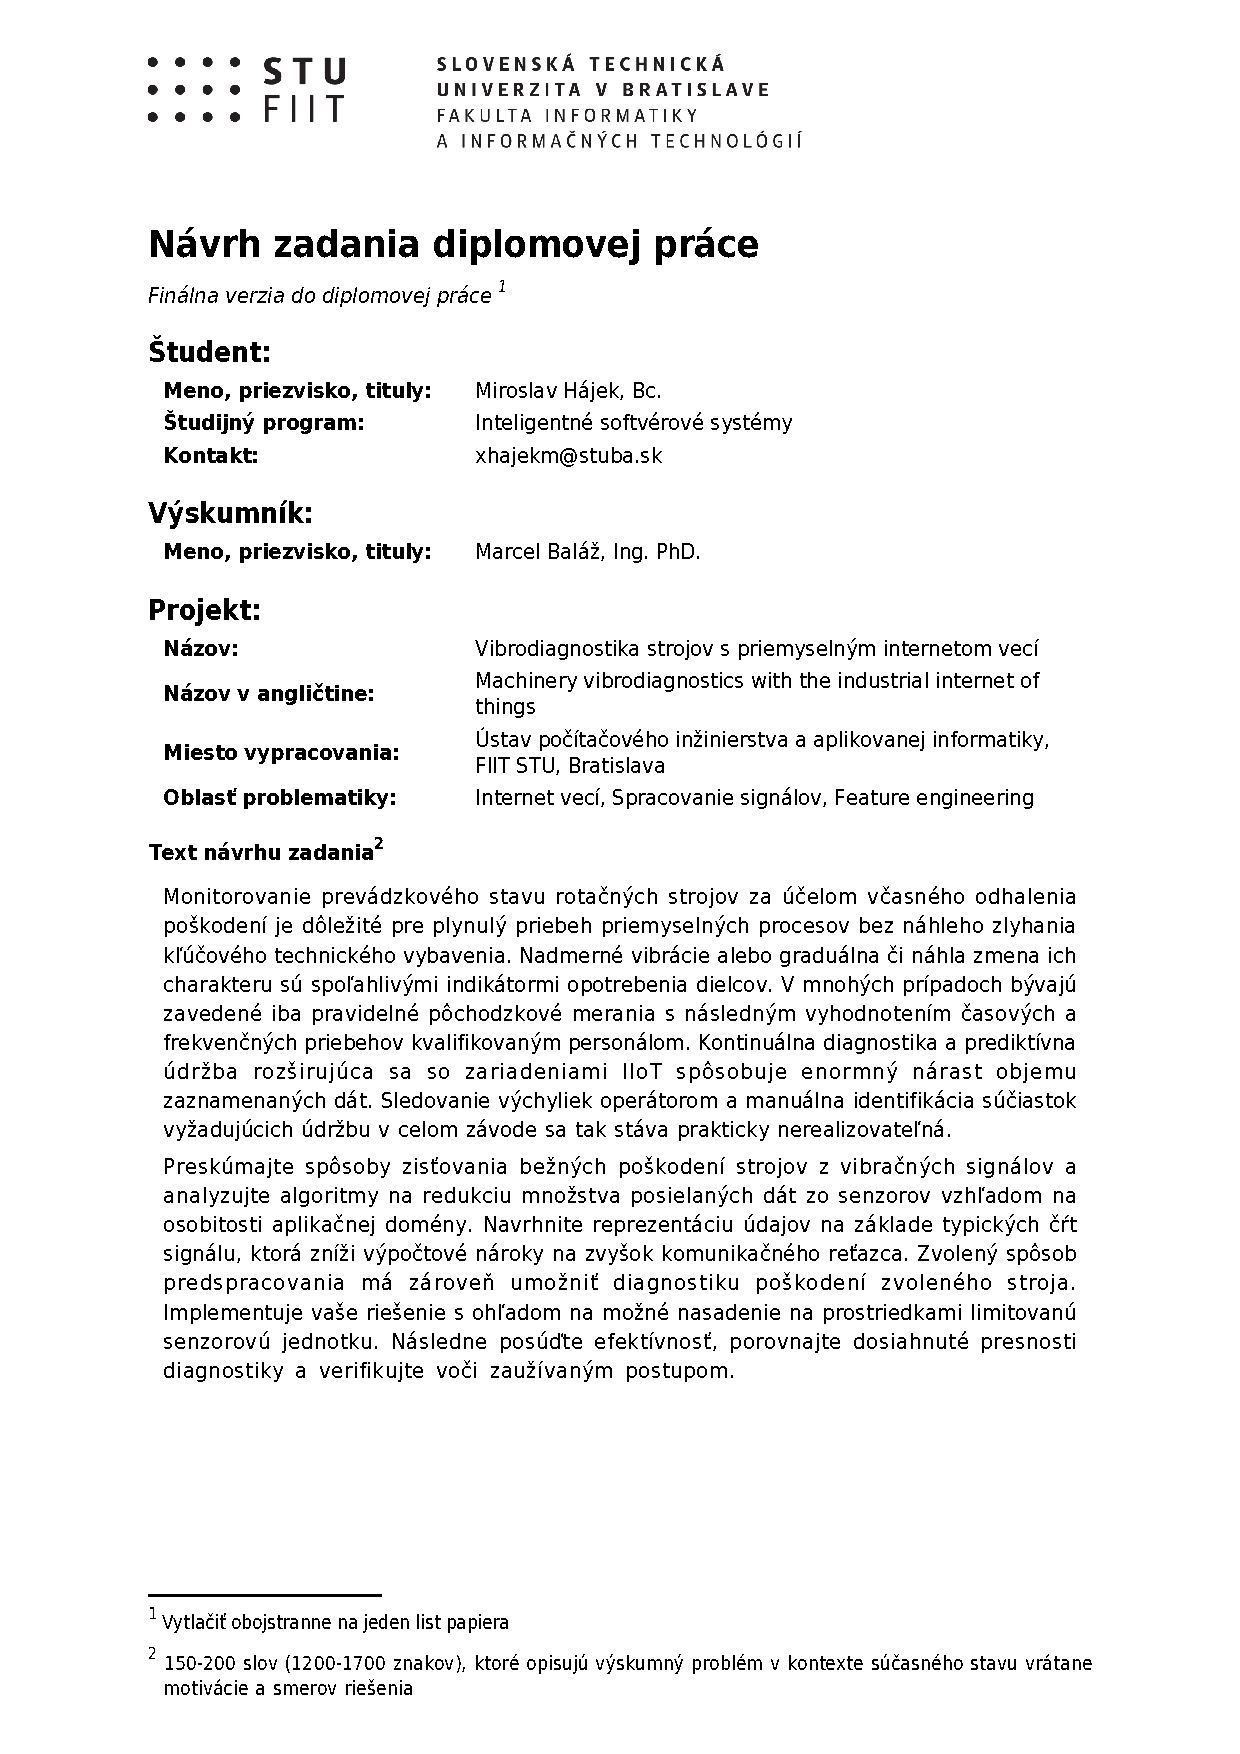
\includepdf[pages=-, scale=1]{chapters/assignment}
\emptypage

 % Declation of Honour
\thispagestyle{empty}
\vspace*{\fill}
\section*{Declation of Honour}

I hereby declare on my honour that I wrote this thesis independently under supervision of Dr. Marcel Baláž, after consultations and with use of cited literature.

\vspace{3\medskipamount}\noindent
\SignPlace \SignDateEN \hspace*{\fill} \signaturespace{5cm}{\Author} 

\emptypage
% Poďakovanie
\thispagestyle{empty}
\vspace*{\fill}
\section*{Acknowledgement}

\vspace{3cm}
\emptypage
\thispagestyle{empty}
\section*{Annotation}
\UniversityEN \\
\uppercase{\FacultyEN}
\vspace{-8pt}
{\setlength{\mathindent}{0cm}
\begin{align*}
&\text{Degree course:} && \text{\StudyProgrammeEN} \\
&\text{Author:} && \text{\Author} \\
&\text{\ThesisEN:} && \text{\TitleEN} \\
&\text{Supervisor:} && \text{\SupervisorEN} \\
&\text{\DateEN}
\end{align*}}

\emptypage 

\thispagestyle{empty}
\section*{Anotácia}
\University \\
\uppercase{\Faculty}
\vspace{-8pt}
{\setlength{\mathindent}{0cm}
\begin{align*}
&\text{Študijný program:} && \text{\StudyProgramme} \\
&\text{Autor:} && \text{\Author} \\
&\text{\Thesis:} && \text{\Title} \\
&\text{Vedúci diplomovej práce:} && \text{\Supervisor} \\
&\text{\Date}
\end{align*}}

\emptypage

% Obsah
\pagestyle{empty}
\tableofcontents{}
\listoffigures
{\let\clearpage\relax \printnomenclature}
\emptypage

\pagestyle{fancy}
% Kapitoly
\pagenumbering{arabic}

\chapter{Introduction}
Manufacturing is experiencing a shift in the traditional practices of asset operational status evaluation and utilization. The rise of Industry 4.0 means greater automation and robotization of the production halls to achieve optimal usage of available resources. The secondary aspect in the enterprises' endeavor, however not less important, is to keep track of the equipment wear and tear. The corrective action be it repair or replacement should be taken on time in response to the key indicators. 

The goal is to preserve required safety and production efficiency when extending the useful life of machine moving parts. In the factories and logistics where this sort of equipment is vital, there is a rising interest in the ability to monitor in real-time the health of the machines and to proactively diagnose the fault to repair it without adding unnecessary costs. 

Vibrations are the most nonintrusive way with which such faults can be sensed. The experts use it to distinguish faulty states and to identify the malfunction's root cause. In critical circumstances such as in the case of the large turbines in the power plants, the precautions leading to regular machinery check-ups are already in place. To reach wider acceptance and spread, the monitoring solution has to be sufficiently independent, reliable, and as self-sufficient as the model design allows it to be.

The main issue to consider in large-scale machinery monitoring using vibrations are lots of uninformative streams of samples not directly useful for the production line operator. The dashboard must aggregate these flows into trend variables with severity levels categorized based on industrial standards. The majority of signals are viewed once at the maximum therefore to store or even transmit them from the edge device in its entirety would be wasteful. The complex overview of the mechanical equipment status is attainable only when agent devices and sensors are cheap enough with a long lifespan on battery power and preferably remain physically small to reduce the additional clutter.

Attempted machine and deep learning approaches have the crucial impediment that the construction of every single machine is unique to some extent because of tolerances and variable load. The model must be trained specifically for the target environment to achieve the ideal performance. In addition, the failures are relatively rare events occurring usually in the span of multiple months. In these circumstances, it is hard to obtain a large enough sample of fault events quickly. Novelty detection is a technique that can be applied in this case.

The thesis is organized in the following manner. In the first chapter of analysis in section 1 we explore the mechanical maintenance approaches and industry standards on common fault identification. Then section 2 is all about measuring vibrations and transforming them into features meaningful in automatic fault pattern recognition. In section 3 we delve into modes of diagnosis based on reduced relevant indicators. Section 4 deals with evaluation datasets used to determine computational requirements
on IIoT infrastructure. Chapter 2 defines data format and proposes processing steps to diagnose the imminent failure and different fault types. The approach taken is evaluated and validated in Chapter 6. 
  

% Ďaľšie kapitoly v zvlášť súboroch
\chapter{Problem analysis}


\section{Condition monitoring}

What are predicted variables - result of diagnoses
\begin{itemize}
\item - Presence of the Fault
\item Type of fault present (different characteristics - e.g. frequency content)
\item Remaining Useful Life (time until failure) - machines of the same type and different degradation curves
\end{itemize}

\textbf{Remainig useful life models} (RUL) - is the expected life or usage time remaining before the machine requires repair or replacement.
\url{https://www.mathworks.com/help/predmaint/ug/rul-estimation-using-rul-estimator-models.html}
\begin{itemize}
\item Similarity - run to failure history of similiar machines in database
\item Degradation - known failure threshold (warning, alert threshold)
\item Survival  - life-span of components and correlated variables
\end{itemize}


\cite{jung_vibration_2017}
\begin{itemize}
\item Indirect Measurement: indirect and approximate measurement over the vibration phenomenon of the target equipment.
\item Noisy and Unaligned Observations: well aligned / may contain huge amount of noise.
\item Variance on Initial Status: initial status of the target equipment different from each other.
\item Diversity on Lifetime model: the usage and lifetime model -  number of unknown and external factors.
\end{itemize}

\subsection{Maintenance strategies}
Difference between fault (degrating performace of the machine - higher friction and power consumption) and failure (machine is unusable). \cite{mohanty_machinery_2015} (picture)
\begin{itemize}
\item Reactive - run equipment until failure occurs - low stakes operation. Failure can have negative economic impact or can damage adjacent parts
\item Preventive - predetermined schedule when assets are diagnosed and repairs are made. Crutial to set appropiate maintanance interval. Good parts are replaced before they are completely worn out, preventing critical failure, but creating unneccesary waste. Sometimes faults are not detected soon enough.
\item Predictive - model of expected lifetime, warns about unexpected faults before they become too serious and before affecting the machine.
\end{itemize}

Wear process curve \cite{mohanty_machinery_2015} Bath tub curve (page 10)
\begin{itemize}
	\item Initial - large roughness
	\item Normal - contact area fomred
	\item Severe - high friction
\end{itemize}

Rotordynamics (chapter 4) (p. 29)  - p.97 - Fault types, p.127 - faults in electric motors

In order to understand, and correctly diagnose the vibratory characteristics of rotating machinery, it is essential for the machinery diagnostician to understand the physics of dynamic motion. This includes the influence of stiffness and damping on the frequency of an oscillating mass — as well as the interrelationship between frequency, displacement, velocity, and acceleration of a body in motion. \cite{eisenmann_machinery_1997}
\begin{itemize}
\item Forced Vibration Mechanism
	\begin{itemize}
	\item Mass Unbalance
	\item Misalignment
	\item 	Shaft Bow
	\item Gyroscopic
	\item Gear Contact
	\item Rotor Rubs
	\item Electrical Excitations
	\item External Excitations
	\end{itemize}
\item Free Vibration Mechanism
	\begin{itemize}
	\item Oil Whirl
	\item Oil or Steam Whip
	\item  Internal Friction
	\item Rotor Resonance
	\item Structural Resonances
	\item Acoustic Resonances
	\item Aerodynamic Excitations
	\item Hydrodynamic Excitations
	\end{itemize}
\end{itemize}

\subsection{Vibration fault types}
There are a few methods of machinery fault identification in vibrational signals based on domain expertise. Data points can be viewed in the time domain and frequency domain. Either as individual stationary profiles obtained during the short duration in the time of measurement, or multiple spaced-out observations with the intent to highlight the long-term trend, e.g. shown in a waterfall plot \cite{ziaran_technicka_2013}. The descriptor variable can be any meaningful statistical quantity, e.g. peak-to-peak, RMS, crest factor, kurtosis, which can be applied to recorded samples or frequency bands.

Mechanical faults manifest themselves in the vibration signal at various frequencies. In the low-frequency range (up to 1 kHz) shaft's unbalance, misalignment, bend, crack, and mechanical looseness is present. High frequencies (up to 16 kHz or more) contain bearings faults and gear faults.

Under fault-free circumstances, shaft speed appears as the strongest frequency component. In case of shaft and gear imbalance or damage, synchronous multiples of shaft frequency (harmonics) are amplified. When rub, bad drive belts and chains, or looseness is occurring in the machine then sub-synchronous harmonics or even non-synchronous frequencies appear \cite{mohanty_machinery_2015}.  Therefore it is useful to rescale the horizontal axis to RPM or orders of rotational speed. Complementary methods of fault symptom identification are phase and orbital analysis \cite{scheffer_practical_2004}.

\begin{itemize}
\item Bearing faults - vibration on each rotation of rolling elements, CFC (characteric fault frequencies with impulse
\item Rotor bar faults - current will not flow - forces diffrent on both sides of rotor
\item Eccentricity Faults - uneven air gap between stator rotor
\item Misalignment - parralel / angular
\item Cavitation - pumps
\item Gearbox fault -broken teeth
\end{itemize}
measuring vibration with current, thermal, flux is improvement, +acoustic elminited (detect similiar faults)
vibration is better alone, then other methods alone (80 vs. <60%)
 \cite{goel_methodology_2022}

\subsection{Technical standards}
The maintenance procedure usually involves data acquisition cards inside handheld devices with accelerometer sensor probes then mounted firmly to the machine frame by either screwing in, magnets or wax \cite{ziaran_technicka_2013}. The probe placement in axial and perpendicular radial directions is standardized in ISO 20816. The severity of vibrations is mostly assessed in units of velocity ($mm/s$), but acceleration ($m/s^2$) and displacement ($\mu m$) are also used. Based on the observed vibration intensity and one of the four classes of machines (I, II, III, IV) by output power and size, zones (A, B, C, D) for accepted levels are proposed. It is customary to establish operational limits in the form of alarms and trips \cite{iso_20816}.

Standard ISO 13373 categorizes three types of vibration monitoring systems: permanent, semi-permanent, and mobile. More importantly, a structured diagnostic approach is developed here complete with recommendations for formalizing diagnostic techniques \cite{iso_13373}. The next step is the signal analysis with the use of proper units and transformations is the subject of the ISO 18431 \cite{iso_18431}.

ISO-10816 Vibration Severity Chart
Typical faults produce unusual low-frequency vibrations (10 to 1000 Hz).
Imbalances, misalignments and looseness are recorded at frequencies up to 300 Hz.

\paragraph{Sensor placement}

\section{Feature engineering}
\subsection{Feature extraction}
Statistical features in Time-domain (and correlation to blade wear) \cite{zhuo_research_2022} \cite{zheng_feature_2018}
\begin{itemize}
	\item 	Root mean square (0.98)
	\item Mean (0.17)
	\item Amplitude (0.81)
	\item Kurtosis (0.042)
	\item Peak to peak (0.463)
	\item Signal strength (0.119)
	\item Standard deviation (0.908)
	\item Peak value (0.488)
	\item Shape factor (0.007)
	\item Skewness (0.118)
	\item Avearge signal level (0.46)
	\item Crest factor (0.056, spikeness of the signal - rms/amplitude)
\end{itemize}
Selection according to high correlation (graph: sawn-trough section vs feature)
Features in time domain with high correlaction: RMS, Standard deviation, Amplitude

Statistical features in Frequency domain (PSD analysis) r >= 0.8 db3 analysis
\begin{itemize}
	\item 	Root mean square (0.402)
	\item Mean (0.497)
	\item Peak frequency (0.670)
	\item Kurtosis (0.852)
	\item Peak to peak (0.076)
	\item Standard deviation (0.799)
	\item Peak value (0.787)
	\item Shape factor (0.851)
	\item Skewness (0.819)
	\item Frequency centroid (0.775)
\end{itemize}
skewness (PSD\_S), kurtosis (PSD\_k), and shape factor (PSD\_Sf),
centroid frequency (FFT\_fc), wavelet packet energy entropy (WPD\_EP) = 0.85
- The WPD energy E8, E10, and E12
- Energy ratios P8 and P13 of frequency bands 8 and 13

Spectral features \cite{peeters_large_2004} - 1. Spectral shape description
\begin{itemize}
\item Coherence function - correlation between two signals PSD
\item  Spectral centroid - barycenter of the spectrum (weighted mean of the frequencies present in the signal, with their magnitudes as the weights)
\item Spectral spread
\item Spectral skewness
\item Spectral kurtosis
\item Spectral slope - comupted with linear regression - amount of decresing of the spectral amplitude
\item Spectral roll-off - 95\% of the signal energy is contained below this frequency
\item 2. Temporal variation of spectrum - spectral flux - correlation of normalized cross-correlation between two succesive amplitude spectra
\end{itemize}

Harmonic features
\begin{itemize}
\item Fundamental frequency  - Maximu likelihood algorithm
\item Noisiness - ratio - energy of noise to the total energy
\item Inharmonicity - energy weighted difference of the spectral components from the multiple of fundamental frequency
\item Harmonic Spectral Deviation - deviation of amplite harmonics peaks from global spectral envelope
\end{itemize}

\textbf{Harmonic peak feature} - \cite{jung_vibration_2017}- group of pairs of significant peaks’ value and frequency in PSD. Harmonic peak distance Dij

\begin{itemize}
\item Standardization - Min-max scaler, Standard scaler (clustering - feature have different scales)
\item Transformation - Log transformation, Box-Cox
\end{itemize}

major drawbacks of PSD
\begin{itemize}
	\item PSD is a highdimensional feature (i.e., 1024 dimensions in our case) that often generates singular matrix = regression algorithms.
	\item PSD feature is unreliable due to a large random fluctuation in their amplitudes over frequency due to measurement noise inherent in MEMS sensor.
\end{itemize}


\subsubsection{Signal denoising and filtering}
Blind source separation, PCA, ICA
vibration analysis tools:
\begin{itemize}
\item ICA (independent component analysis),
\item TFA (time-frequency analysis),
\item ED (energy distribution) and
\item CD (change detection)
\end{itemize}

\subsubsection{Time-frequency features}
The PSD is the overall expectation of the AE signal. It needs to be calculated by estimation methods. The estimation of the power spectrum is realized by Welch method (cite)

Time Synchronous Averaging of Real FFT
vs. FastCWT - Synchrosqueezing

\subsubsection{Harmonics identification}
Cepstrum + Harmonic Product Spectrum + Peak identification


\subsection{Feature selection}
Feature importance ranking of Numeric features - Filtering
\begin{itemize}
\item High correlation with predictor - band saw blade width of flank face --- to signal statistics
\item Low correlation (Decorrelation) among predictors themselves - if they are correlated they produce same response
\item ANOVA with F-Test - Variance of the feature - high variance - is high response
\item Linearly dependent features are a waste of space and computation power because the information could have been encoded in much fewer features. \cite{zheng_feature_2018} - solve by PCA
\end{itemize}

Vibration levels are dependent on the type of work (load) of the machine (cite)
\begin{itemize}
\item \textbf{Sawing process database}: it contains basic information such as sawing machine tools model, band saw blade model, sawing parameters, and the material and size of the workpiece to match the relevant online monitoring model.
\item \textbf{Online monitoring model database}: it stores online monitoring models of band saw blade wear based on different sawing processes.
\end{itemize}

\section{Diagnostics techniques}
\url{https://scikit-learn.org/stable/modules/outlier_detection.html#outlier-detection}
\subsection{Novelty detection}
\textbf{Fault or no fault} - anomaly detection solutions - unsupervised \cite{torres_automatic_2022}. mean shift clustering algorithm
\begin{itemize}
\item Robust Covariance  (Mahalanobis distance)
\item One-class SVM with non-linear kernel (RBF) - classifying new data as similar or different to the training set
\item Local outlier factor - local density deviation of a given data point with respect to its neighbours
\item Isolation forest
\end{itemize}

\textbf{Types of faults - clustering}
\begin{itemize}
\item BIRCH
\item DBSCAN - density based params:
	minPts (the minimum number of data points that need to be clustered together for an area to be considered high-density)
	eps (the distance used to determine if a data point is in the same area as other data points).
\item OPTICS - better DBSCAN -  clusters in data of varying density
\end{itemize}

\subsection{Label propagation in semi-supervised learning}

Transductive Support vector machine(TSVM),
Label Propagation Algorithm(LPA)

\section{IoT in Industry 4.0}
	Wireless protocols limitation: IEEE 802.11, IEEE 802.15.4e, OpenThread
	Power consumption
	Devices and sensors

	The Fig. 1 shows a generalist architecture supported in the context of Industry 4.0, fault detection systems in electrical machines based on vibration analysis  The Operational Technology (OT) and Information Technology (IT) parts were aligned to design an Industrial Control System (ICS) in the laboratory, for acquiring, controlling and monitoring the operating status of rotating machines, producing reports, automatic alerts and recommending actions to take as a prescriptive maintenance system. \cite{torres_automatic_2022}


\nocite{*}
\printbibliography[heading=bibintoc, title={Literature}]

%  Prílohy -----------------------------------------------------------------------
\addtocontents{toc}{\protect\setcounter{tocdepth}{0}}
\addtocontents{toc}{\cftpagenumbersoff{chapter}}
\let\svaddcontentsline\addcontentsline
\renewcommand\addcontentsline[3]{%
  \ifthenelse{\equal{#1}{lof}}{}%
  {\ifthenelse{\equal{#1}{lot}}{}{\svaddcontentsline{#1}{#2}{#3}}}}

\appendix
\titleformat{\chapter}{\normalfont\huge\bf}{Appendix \thechapter:}{1em}{}
\renewcommand{\chaptermark}[1]{\markboth{\MakeUppercase{Appendix \thechapter.\ #1}}{}}

\thispagestyle{empty}
\chapter{Resume}
\pagenumbering{arabic}
\renewcommand*{\thepage}{A-\arabic{page}}


\clearpage


\thispagestyle{empty}
\chapter{Plan of work}
\pagenumbering{arabic}
\renewcommand*{\thepage}{B-\arabic{page}}

\section{Winter semester}

\begin{table}[h!]
\def\arraystretch{1.25}
\begin{tabular}{|l|p{12cm}|}
\hline
\textbf{Period} & \textbf{Work}                                                                                                                                                                                                                         \\ \hline
\nth{1} week         & Consultation with the supervisor on directions of the future work based on literature review during previous semester.
\\ \hline
\nth{2} week         & Outline the key sections of the analysis part in the thesis.
\\ \hline
\nth{3} week         & Match supporting literature with analysis sections. Further invesigation on the feature engineering methodology in condition monitoring.
 \\ \hline
\nth{4} week         & Summarize notes from condition monitoring articles and videorecordings of tutorials and conferences.
 \\ \hline
\nth{5} week         & Research transformation of vibration signal to feature space using time-frequency, harmonic and energy statistical metrics. Progress report meeting with the supervisor.
 \\ \hline
\nth{6} week         & Find articles and take notes about unsupervised and semi-supervised techniques in streaming data for machinery diagnostics, in order to gather information about suitable features.
 \\ \hline
\nth{7} week         & TBD (Narrow down wide variety applicable methods for signal decomposition)
 \\ \hline
 \nth{8} week         & TBD (Write thesis section on condition monitoring and machinery fault types)
 \\ \hline

\end{tabular}
\end{table}

\clearpage
\newpage


\section{Summer semester}

\clearpage


% Ďalšie prílohy
% \input{chapters/appendix/B-technical-docs}
% Ak nechce vypísať čísla strán na konci prílohy: \cleardoublepage

\thispagestyle{empty}
\setcounter{figure}{0}
\chapter{Digital medium}
\pagenumbering{arabic}
\renewcommand*{\thepage}{C-\arabic{page}}
\par Evidenčné číslo práce v informačnom systéme: \RegNo
\par Obsah digitálnej časti práce (archív ZIP):
\par Názov odovzdaného archívu: 



\end{document}
